\documentclass[border=10pt]{standalone}
\usepackage{tikz}
\usetikzlibrary{arrows.meta, shapes, calc}

\begin{document}
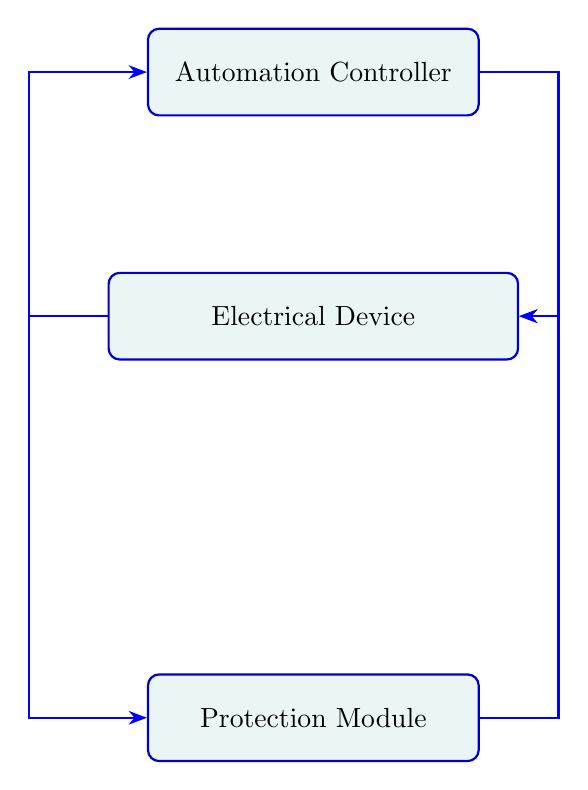
\begin{tikzpicture}[
    node distance=2cm,
    block/.style = {rectangle, draw=blue!80!black, thick, rounded corners, fill=teal!8, minimum width=4.2cm, minimum height=1.1cm, align=center},
    arrow/.style = {thick, blue, -Stealth}
]

% Place the nodes
\node[block] (controller) at (0, 2) {Automation Controller};
\node[block, minimum width=5.2cm] (device) at (0, -1.1) {Electrical Device};
\node[block] (module) at (0, -6.2) {Protection Module};

% Draw side-routed bidirectional arrows between adjacent blocks
\draw[arrow] (device.west) -- ++(-1.0,0) |- (controller.west);
\draw[arrow] (controller.east) -- ++(1.0,0) |- (device.east);
\draw[arrow] (device.west) -- ++(-1.0,0) |- (module.west);
\draw[arrow] (module.east) -- ++(1.0,0) |- (device.east);

\end{tikzpicture}
\end{document}
